\documentclass[10pt]{article}
\usepackage[usenames]{color} %used for font color
\usepackage{amssymb} %maths
\usepackage{amsmath} %maths
\usepackage[ruled,linesnumbered]{algorithm2e}
\usepackage[utf8]{inputenc} %useful to type directly diacritic characters

\usepackage{graphics}
\usepackage{adjustbox}
\usepackage{float}
\usepackage{listings}



\begin{document}





\textnormal{
Describe a User Interface (UI) to your application along with the related information that will be shown on each interface view (How users will query or navigate the data and view the query or navigation results). The emphasis should be placed on the process a user needs to follow in order to meet a particular information need in a user-friendly manner.
The deliverables for this stage include the following items :\\\\
Section 1: The UI for finding semantic similar tweets based on Edit Distance integrated Word2Vec (EDW) and K-medoids clustering (implemented by Lingfei Zeng).\\\\
The mode of user interaction with the data is text queries and mouse clicks. There are two input boxes. The first one is for text input such as a tweet, some key word or a topic (such as hashtags in tweets). The second one is for an integer to indicate how many (top) similar tweets one would like to display. Then mouse click for submit, the UI will return the output, which are the similar tweets. \\\\
The initial UI screenshot in shown Figure \ref{fig1}. After input a tweet and the number of tweets one like to show, the result is shown in Figure \ref{fig2} and Figure \ref{fig3} . One can also input one word as topic or hashtags in the tweets. The search result is shown in  Figure \ref{fig4}. Overall, the output is quite accurate, which indicates the good performance and versatility of our algorithm. \\\\
The error massage will pop out if user does not input anything but hit submit button. It's shown in Figure \ref{fig5}.   
}

 
\begin{figure}[h]
	\caption{Initial UI screen shot}
	\centering
	
\includegraphics[scale=0.3]{Screen_Shot_1.png}
	\label{fig1}
\end{figure}

\begin{figure}[h]
	\caption{Output after input of a tweet}
	\centering
	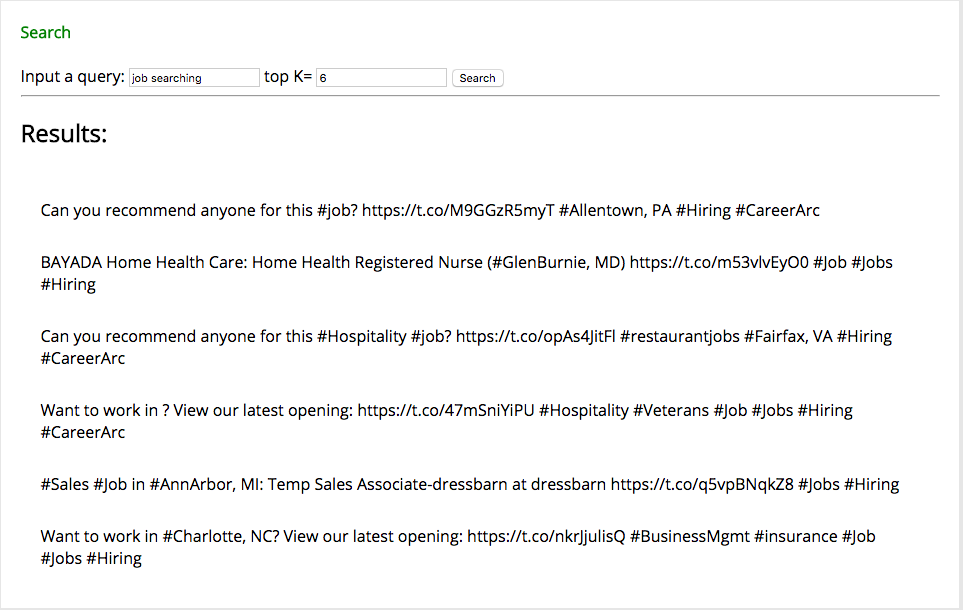
\includegraphics[scale=0.3]{Screen_Shot_2.png}
	\label{fig2}
\end{figure}

\begin{figure}[h]
	\caption{Output after another tweet}
	\centering
	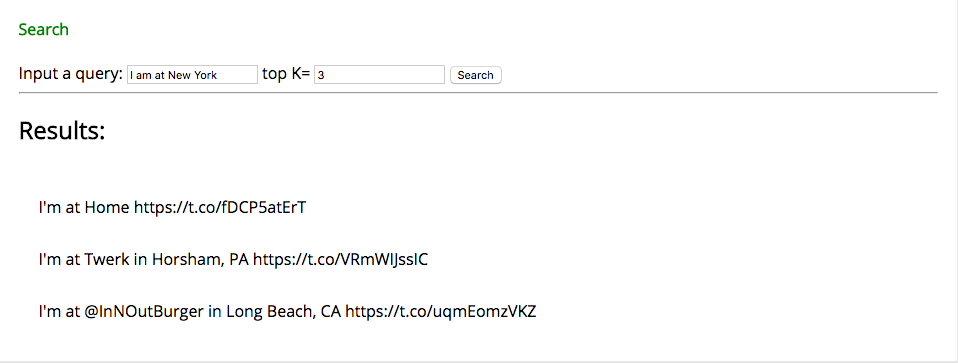
\includegraphics[scale=0.3]{Screen_Shot_3.png}
	\label{fig3}
\end{figure}

\begin{figure}[h]
	\caption{Output after input a hashtag}
	\centering
	\includegraphics[scale=0.3]{Screen_Shot_4.png}
	\label{fig4}
\end{figure}

\begin{figure}[h]
	\caption{Error message when user doesn't input query but hit the submit button }
	\centering
	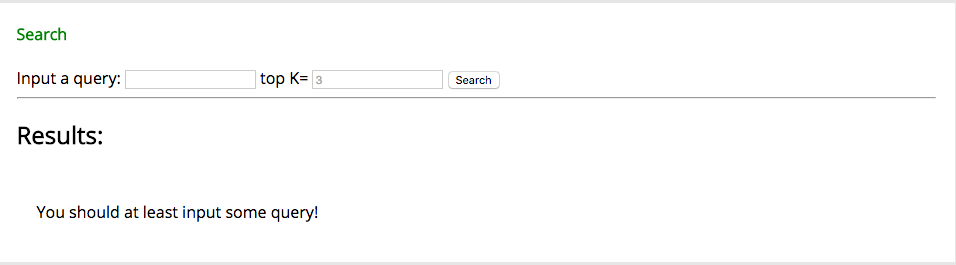
\includegraphics[scale=0.3]{Screen_Shot_5.png}
	\label{fig5}
\end{figure}

\end{document}
